%%%%%%%%%%%%%%%%%%%%%%%%%%%%%%%%%%%%%%%%%%%%%%%%%%%%%%%%%%%%%
%% HEADER
%%%%%%%%%%%%%%%%%%%%%%%%%%%%%%%%%%%%%%%%%%%%%%%%%%%%%%%%%%%%%
\documentclass[a4paper,twoside,10pt]{article}
% Alternative Options:
%	Paper Size: a4paper / a5paper / b5paper / letterpaper / legalpaper / executivepaper
% Duplex: oneside / twoside
% Base Font Size: 10pt / 11pt / 12pt

%% Language %%%%%%%%%%%%%%%%%%%%%%%%%%%%%%%%%%%%%%%%%%%%%%%%%
\usepackage[USenglish]{babel} %francais, polish, spanish, ...
\usepackage[T1]{fontenc}

%\usepackage[ansinew]{inputenc}
\usepackage[utf8]{inputenc}	%supports Umlaute
\usepackage{german, ngerman}
\usepackage{eurosym}
\usepackage{color}

\usepackage{lmodern} %Type1-font for non-english texts and characters

%% Packages for Graphics & Figures %%%%%%%%%%%%%%%%%%%%%%%%%%
\usepackage{graphicx} %%For loading graphic files
%\usepackage{subfig} %%Subfigures inside a figure
%\usepackage{tikz} %%Generate vector graphics from within LaTeX

%% Math Packages %%%%%%%%%%%%%%%%%%%%%%%%%%%%%%%%%%%%%%%%%%%%
\usepackage{amsmath}
\usepackage{amsthm}
\usepackage{amsfonts}

%% Other Packages %%%%%%%%%%%%%%%%%%%%%%%%%%%%%%%%%%%%%%%%%%%
\usepackage{a4wide} %%Smaller margins = more text per page.
\usepackage{fancyhdr} %%Fancy headings
%\usepackage{longtable} %%For tables, that exceed one page

\usepackage[parfill]{parskip} 

%%%%%%%%%%%%%%%%%%%%%%%%%%%%%%%%%%%%%%%%%%%%%%%%%%%%%%%%%%%%%
%% DOCUMENT
%%%%%%%%%%%%%%%%%%%%%%%%%%%%%%%%%%%%%%%%%%%%%%%%%%%%%%%%%%%%%
\begin{document}

%\setlength{\parindent}{0pt} %kein Einzug beim Absatzbegin
\pagestyle{fancyplain}

%\title{Aufgabenblatt 3 - Trading Agent Competition} 
%\author{Tiare Feuchtner, Marcel Karsten}
%\date{Abgabetermin: 11.12.2011} %%If commented, the current date is used.
%\maketitle

\rhead{TU Berlin - MPI, WS2012/13}
\lhead{Tiare Feuchtner, Marcel Karsten}
\renewcommand{\headrulewidth}{0px}
%%%%%%%%%%%%%%%%%%%%%%%%%%%%%%%%%%%%%%%%%%%%%%%%%%%%%%%%%%%%%

\begin{center}
\huge{\textbf{Assignment 3 - Fitts' Law}}
\end{center}
\vspace{.5cm}

\section{Fitts' Law Optimization} 
\subsection{Fitts' Law Examples} 
Following are three examples where Fitts' law is applicable in real life or in interaction with a computer.\\
	1. Driving a car: In a car with manual gear shift, the brake and accelerator are alternately pressed with the right foot. These pedals often vary in size and also in distance to each other, depending on the make and type of car. For instance a truck will have significantly larger pedals, compared to a compact car, and in a sportscar, the pedals will be closer together and also have less leverage path. These characteristics could be defined as the width W and distance D of a target, to evaluate the situation with Fitts' law.\\
	2. In the webbrowser Firefox, the conception of the Back button has changed somewhat after version 8 \ref{jaws}. As opposed to then, the clickable area has been enlarged, and now includes the area between the button and the left screen bordern. The larger target facilitates clicking it and placement at the border allows fast and less precise momevent to reach it. \\ 

\begin{figure}[h]
	\centering
		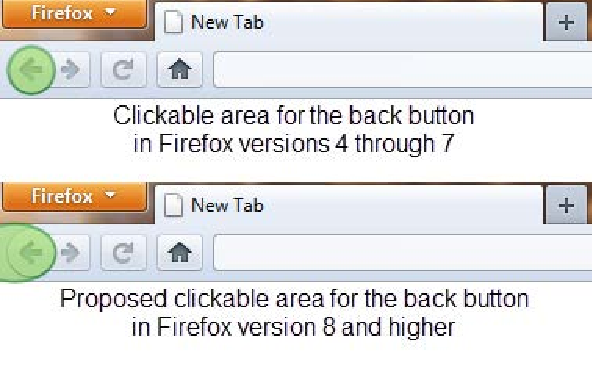
\includegraphics[width=0.50\textwidth]{firefox.pdf}
	\caption{Firefox back button: Increase of clickable area \ref{jaws}}
	\label{fig:firefox}
\end{figure}

	3. The usual context menu which appears by right mouseclick performs quite well when evaluated with Fitt's, since it appears directly at the mouse position. This makes the path to the desired option quite short. However it could still be optimized, as can be seen in the following image \ref{azu}. If the menu would surround the mouse pointer in a circle, instead of being a list, the distance D to each option could be minimized. Also the accuracy of hitting each target could be adjusted by increasing the width of the circle, and thus also the width of each button.

\begin{figure}[h]
		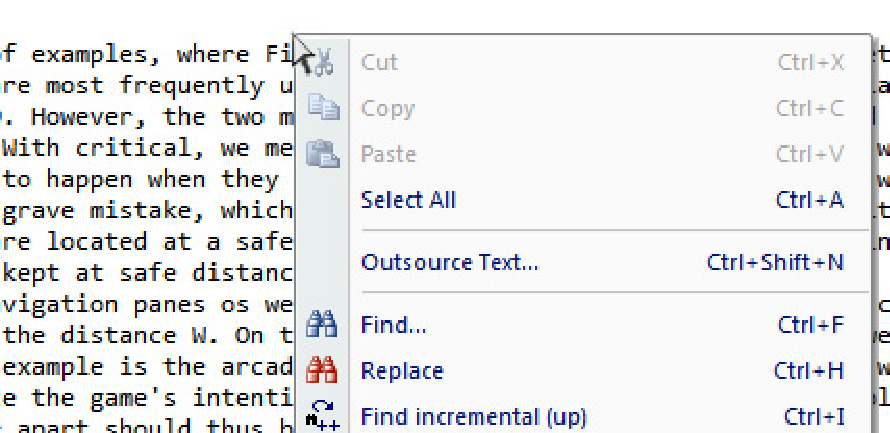
\includegraphics[width=0.40\textwidth]{context_menu.pdf}
	\caption{Traditional context menu}
	\label{fig:context_menu}
\end{figure}

\begin{figure}[h]
	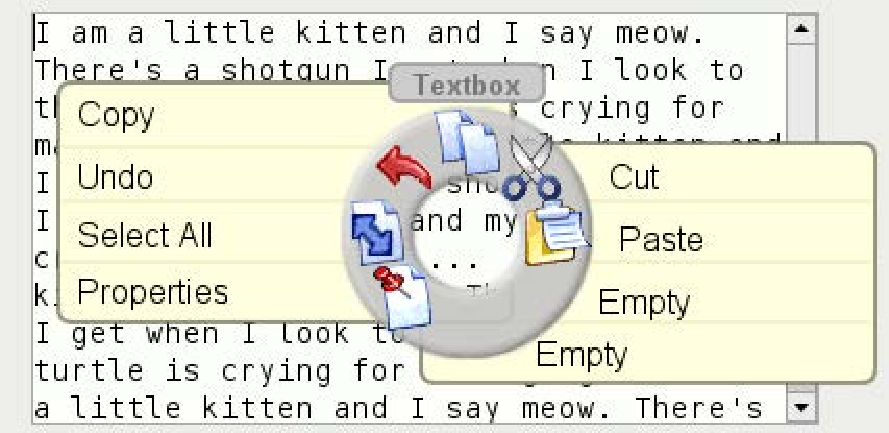
\includegraphics[width=0.40\textwidth]{pie_textbox.pdf}
	\caption{Pie context menu \ref{azu}}
	\label{fig:pie_textbox}
\end{figure}


Following are a couple of examples, where Fitt's law does not apply. First of all let's look at an email client. According to Fitt's law, the buttons which are most frequently used, should be the most prominent with large W and would optimally be positioned close to each other to minimize D. However, the two most popular functions here are Reply and Delete, which have quite unrelated and even critical functionality. With critical, we mean, that the unintentional click on the wrong button could have a very negative outcome amd this is more likely to happen when they are close together. So if for instance, we wish to reply to an email, but click on Delete instead, we have made a grave mistake, which requires the functionality of undoing it. Thus many email clients are designed in a way that these two buttons are located at a safe distance, as can be seen in the following figure. [figure] Similarly an Accept and Cancel button should be kept at safe distance.\\
Further there are the navigation panes os websites, which fold out on hover or when clicked, to reveal more targets. This significantly increases the distance W. On the other hand, it helps organize large websites which has an even more important effect.\\A somewhat less serious example is the arcade game Wack-A-Mole, where you hit moles with a hammer when they stick out their heads from their burrows. Since the game's intention is to make it difficult to hit the moles it will try to break with Fitts' law. Small mole heads appearing par apart should thus be favored.

\subsection{Keyboard redesign} 
Calculating the average movement time MT of pointing to the keyboard and then pointing to the call button.

$MT_1$ ... average Movement Time (old design) \\
$MT_2$ ... average Movement Time (new design) \\
$W = 5$ ... target width (call button or center of keypad) \\
$D_1 = 35$ ...  target distance (old design) \\
$D_2 = 15$ ... target distance (new design) 

$a$ ... start/stop time of device (intercept) \\
$b$ ... inherent speed of device (slope) \\
$ID$ ... index of difficulty

General formula: \\
$MT = a + b \cdot ID$ \\
$MT = a + b \cdot log_2 (1 + \frac{D}{W})$ 

Calculation: \\
$MT_1 = a + b \cdot log_2 (1 + \frac{35}{5}) = a + b \cdot log_2(8) = a + 3b$ \\
$MT_2 = a + b \cdot log_2 (1 + \frac{15}{5}) = a + b \cdot log_2(4) = a + 2b$ \\
Result: $MT_2 = MT_1 - b$ \\
The movement time difference between the two designs is $b$, which clearly rates the new design better.

\section{Fitts' Law Evaluation}
The three devices to be tested, are the laptop's own touchpad, and external mouse and finally a Wacom tablet. The following nine trials have been repeated on each of these.
results of all 3 experiments --> screenshots of the 9 targets\\

The following figures show the resulting graphs obtained with each of the three devices. Further details about the performance of each device are contained in the table below.

Experiment 1: Touchpad --> Screenshot of result\\
Experiment 2: Mouse --> Screenshot of result\\
Experiment 3: Tablet / different User? --> Screenshot of result



%\subsection{Resultate}
%Das Walverine-System vermag besonders am Anfang des Spiels sehr gute Ergebnisse zu erzielen. In den weiteren Biet-Runden fällt Walverine jedoch zurück, da die Algorithmen mit welchen gearbeitet wird, die Umweltfaktoren zu wenig berücksichtig. So sollte beispielsweise berücksichtigt werden dass die Agenten mit ihren Aktionen die Preise beeinflussen 

\vspace{1cm}

%\textbf{Referenz}\\
%Shih-Fen Cheng Evan, Evan Leung, Kevin M. Lochner, Daniel M. Reeves, L. Julian Schvartzman,
%and Michael P. Wellman. Walverine: A walrasian trading agent. In Second International
%Joint Conference on Autonomous Agents and Multi-Agent Systems, pages 465–472, 2002.

\end{document}
